\documentclass[conference, a4paper, twocolumn]{IEEEtran}
\IEEEoverridecommandlockouts
\makeatletter
\newcommand{\linebreakand}{%
  \end{@IEEEauthorhalign}
  \hfill\mbox{}\par
  \mbox{}\hfill\begin{@IEEEauthorhalign}
}
\makeatother


% The preceding line is only needed to identify funding in the first footnote. If that is unneeded, please comment it out.
%\usepackage{cite}
\usepackage{amsmath,amssymb,amsfonts}
%\usepackage{algorithmic}
\usepackage{algorithm} 
\usepackage{algpseudocode} 
\usepackage{graphicx}
\usepackage{textcomp}
\usepackage{xcolor}
\usepackage{listings}
\usepackage{hyperref}
\usepackage{geometry}
\usepackage{multirow}
\usepackage{tabularx}
\usepackage[
backend=biber,
style=numeric-comp,
sorting=ynt
]{biblatex}
\usepackage{float}
\usepackage{changepage}

\addbibresource{./biblio.bib}
\graphicspath{ {./assets/} }

% If not
\algnewcommand\algorithmicnot{\textbf{not}}
\algdef{SE}[IF]{IfNot}{EndIf}[1]{\algorithmicif\ \algorithmicnot\ #1\ \algorithmicthen}{\algorithmicend\ \algorithmicif}

% Line comment
\algnewcommand{\LineComment}[1]{\State \(\triangleright\) #1}

\def\BibTeX{{\rm B\kern-.05em{\sc i\kern-.025em b}\kern-.08em
    T\kern-.1667em\lower.7ex\hbox{E}\kern-.125emX}}

% Listings style
\lstdefinelanguage{pseudo}{
    basicstyle=\small\ttfamily,
    numbers=left,
    numberstyle=\scriptsize,
    stepnumber=1,
    numbersep=8pt,
    showstringspaces=false,
    breaklines=true,
    % frame=lines,
    numbers=left,
    xleftmargin=2em,
    % frame=single,
    % framexleftmargin=1.5em
}

% \geometry{footskip=0.5cm}


\begin{document}

\title{Pedestrian Traffic Analysis of Trindade's Station\\}

\author{\IEEEauthorblockN{Eduardo Correia}
\IEEEauthorblockA{\textit{Faculty of Engineering of University of Porto} \\
up201806433@up.pt}
\and
\IEEEauthorblockN{Henrique Sousa}
\IEEEauthorblockA{\textit{Faculty of Engineering of University of Porto} \\
up201906681@up.pt}
\linebreakand
\IEEEauthorblockN{Mª Francisca Almeida}
\IEEEauthorblockA{\textit{Faculty of Engineering of University of Porto} \\
up201806398@up.pt}
}

\maketitle

\thispagestyle{plain}
\pagestyle{plain}

\begin{abstract}
Rush hour embarking and debarking at a transit platform can cause the intersection of large masses of people, making it harder for easy movement and arriving at the destination. A good design of a multi-modal transit station might help to attenuate this problem, bringing improvements in metrics such as mean average time to changing lines and, more subjectively, stress induced in passengers.
We develop and describe a simulation in Netlogo that is tested in the Trindade, Porto, multi-modal transit station. Multiple scenarios are considered to exemplify its usefulness in evaluating changes to the infrastructure.


\end{abstract}

\begin{IEEEkeywords}
modeling, system modeling, pedestrian traffic
\end{IEEEkeywords}
\section{Introduction} \label{sec:introduction}
% In urban landscapes, the convergence of large crowds during rush hours at transit platforms often results in challenges for efficient movement and timely arrival at destinations. The intricate dynamics of embarking and debarking passengers create bottlenecks that hinder the overall transit experience. This phenomenon not only affects quantitative metrics such as mean average time to change lines but also contributes to the subjective stress experienced by passengers. Addressing this issue requires a strategic approach to the design of multimodal transit stations. 

% This study aims to explore design alternatives for an idealized or specific multimodal transit station with a particular focus on minimizing alterations costs while maximizing improvements in passenger movement. We modelled Trindade Metro station, which is the central metro station in Porto, since is close to the city center, is the point of intersection of all the metro lines, and has access to several bus stations with different lines.

% By delving into the intricacies of station design, we seek to identify practical solutions that enhance the overall transit experience during peak hours, offering a harmonious balance between efficiency and minimalistic alterations.

Public transportation represents one of the most efficient ways to move large masses of people. Large multi-modal transit stations, where multiple modes of transportation coexist, have a lot of pedestrian traffic. Rush hour embarking and debarking between platforms, stops, or bays has large masses of people crossing each other and navigating the station space, often in directly opposite directions. It is in this overall context that a station with multiple floors serving multiple train platforms becomes an interesting problem, for it poses optimization problems not only in scheduling but also in the design of the station itself for faster traveling and cheaper maintenance and construction. \\
In the following work, we attempt to create a simulation of that scenario. We emphasize developing natural path-finding algorithms, particularly across multiple floors, in a computationally efficient way. Collisions between passengers are also taken into account. The developed model also attempts to generalize as much as possible, allowing for different scenarios to be tested easily and changing of parameters. \\

In \autoref{sec:related_work}, we mention some projects related to the pedestrian traffic problem, particularly in subway stations. In \autoref{sec:methods_materials}, we outline the main implementation details and thought process. In \autoref{sec:results_discussion}, we analyze multiple simulated scenarios by changing the environment and the running parameters. Finally, in \autoref{sec:conclusion}, we lay out the conclusions of the work and future work.

\section{Related work} \label{sec:related_work}

With the increasing demand for public transportation, as city centers grow in population, subway stations have to adapt to accommodate the flow of all the passengers with minimal impediments.

As such, several projects exist regarding the simulation of pedestrian flow in stations as a means to analyze different phenomena and alternative scenarios before carrying out any changes to existing stations.

Some examples of successful stories include the Plaça de Catalunya Station \cite{catalunya}, which was remodeled according to a chosen design out of four after using the simulation software LEGION to analyze the most critical metrics. 

In the same fashion, a similar project was conducted for Moscow's metro \cite{moscow}, the busiest in Europe. A model was developed that reflected passenger flow from disembarking from one platform to another and calibrated using real-life data. Ultimately, a proposed solution to change the station topology was accepted.

Examples like these show how useful and insightful simulation and modeling are for optimizing traffic flow in railway stations. Their success boosts the validation of our project, and as such will be used as role models for our project.
\section{Materials \& Methods} \label{sec:methods_materials}

\subsection{Problem formalization}

The transit station will be modeled with the following entities:
\begin{itemize}
    \item \textbf{Floors}, each being a grid with the same size
    \item \textbf{Platforms}, part of a floor
    \item \textbf{Passengers}
    \item \textbf{Points of interest}, either a train or the outside
    \item \textbf{Portals}, either a stair (in practice, representing the top of the stairs) or an elevator
    \item \textbf{Obstacles}, representing walls, train tracks, or other fixtures (benches, trash bins, card validators).
    \item \textbf{Escalators}, either upwards or downwards
\end{itemize}

A floor is made up of one or more platforms. A platform is such that a passenger can get to any place on the platform directly, and other platforms are only accessible by changing floors (taking a portal). \\
Every entity is on a floor at any given point. Passengers can move to other floors by using portals. Different portals can have different behaviors. \\
A passenger spawns in a cell of a point of interest: its source. A passenger has as a destination: a cell of another point of interest. A passenger has a given radius and speed. Two passengers can collide with each other if they are too close. \\
If two portals of the same type are linked, they allow passengers to transition between the respective floors. \\
Using stairs, passengers transition between floors instantly. Using elevators, passengers transition between floors in a time proportional to the number of floors traveled. For simplicity, elevators are static and not dynamic entities. As such, there is no capacity and no floor where the elevator is. When reaching an elevator, a passenger can use it as if it were their own personal elevator.\\
Passengers cannot move through or be too close to obstacles.\\
Every part of a floor that isn't an escalator or an obstacle is deemed as \textit{normal ground}.\\
Escalators provide an increase in passenger speed. An escalator has three logical parts: entry, body, and exit. A passenger can only move to the entry from the normal ground or any escalator's exit and, from there, can only move to the body. A passenger can only move to the body from the entry and, from there, can only move to the exit. A passenger can only move to the exit from the body and, from there, can go to normal ground or any escalator's entry. We will call \textit{moving restrictions} the conditional movement set by escalators.\\
Every entity but the passenger is considered as being the environment. Points of interest and portals are henceforth referred to as static entities. Static entities are made up of several cells. A static entity has a centroid, which is one of its cells. The centroid is the patch used for all of the path-finding operations (see \autoref{sec:methods_materials_static_pathfinding})\\

\subsection{Materials}

The described model was developed in the context of the simulation tools used for this work: NetLogo \cite{netlogo}. \\
Additionally, the Trindade station, the main hub of the subway system of the city of Porto, Portugal, was modeled. Two pictures from its emergency evacuation plan and data collected from Google Maps were used to get a to-scale color-coded image representation of the station to be fed as the simulation's environment. Each color represents one of the aforementioned environmental entities.

\newpage

\subsection{Pipeline}

The simulation happens as follows:
\begin{enumerate}
    \item Prepare the environment
    \begin{enumerate}
    \item Loading of the image. The colors are transformed into variables and data structures within the simulation.
    \item For every platform, initialize the path-finding between static entities
        \begin{enumerate}
            \item Link corresponding portals
            \item Path-finding is done bidirectionally between every distinct pair of the aggregate of points of interest and portals (\autoref{equation:bidirectional_pathfinding}) \\
        \end{enumerate}
            \end{enumerate}
    \item Prepare the simulation run
    \begin{enumerate}
        \item Spawn the passengers one by one
            \begin{enumerate}
                \item Spawn the passenger in a random cell from all of the cells of the points of interest
                \item Choose the destination from the cells of all of the other points of interest
                \item Calculate the shortest path to be taken by the passenger through the different floors.
            \end{enumerate}
    \end{enumerate}
    \item Run the simulation
    \begin{enumerate}
        \item For all passengers
        \begin{enumerate}
            \item Move the passengers to the next point of their path
            \item Collide the passengers between each other
            \item Repel passengers from walls
            \item Log data
            \item Update passengers' path
        \end{enumerate}
    \end{enumerate}
    \item Save data to a file
\end{enumerate}

\begin{equation} \label{equation:bidirectional_pathfinding}
\resizebox{\columnwidth}{!}{
    $\forall{a, b}\ pathfind\left(a, b\right): a, b \in \left(PoI\ \bigcup\ Portals\right) , a \ne b$
}
\end{equation}

\subsection{Platforms and floors}
A transit station is often made up of multiple floors. We didn't use the 3D version of NetLogo for the work as the environment isn't truly three-dimensional but could instead be considered as multiple, discrete, connected 2D layers. Therefore, the image representation of the station is a series of same-sized rectangles of the subsequent floors. \autoref{fig:multiple_floors} represents an example of a station with three floors and four platforms.

\begin{figure}[H]
    \centering
    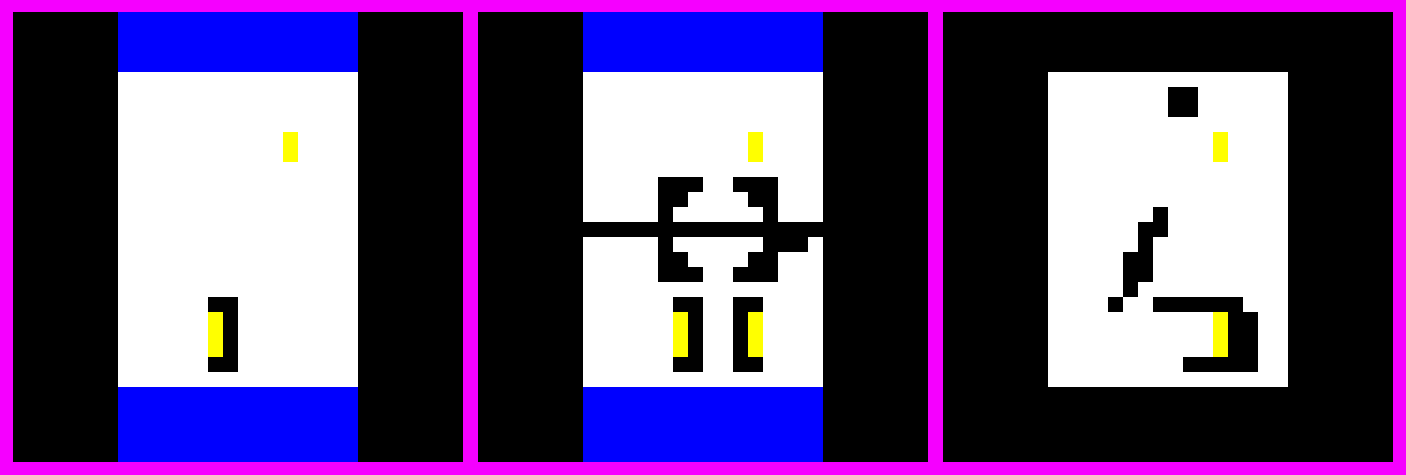
\includegraphics[width=\columnwidth]{assets/multiple_floors.png}
    \caption{Image representation of a station with three floors with obstacles (black), stairs (yellow), and train tracks (blue). The floors are separated by boundaries (pink). The middle floor has two platforms}
    \label{fig:multiple_floors}
\end{figure}

\subsection{Static path-finding}\label{sec:methods_materials_static_pathfinding}

Static path-finding is done for each platform for the centroids of the static entities that belong to it and between the portals that connect platforms. In the end, there are a series of complete bidirectional graphs between the static entities of each and every platform and bidirectional edges connecting those. 

What we describe as path-finding for the portals is as simple as comparing the coordinates of the portal within a floor and matching it to others whose coordinates are the same. We didn't consider the possibility of a transit station with more floors that might have, for example, stairs in the same position but only connecting floors 1 to 2 and 3 to 4, but not 2 to 3. Floor adjacency could be introduced to tackle this issue.

Path-finding for the static entities is the conventional space traversal, which we will now analyze in depth. \\

In NetLogo, there is both a cellular automaton and Euclidean space approach. There are patches, which occupy a quadrangular space with a side of one unit, and turtles that can have \textit{(x,y)} real coordinates that are, nonetheless, heavily linked to the patch (or cell) they are in.  \\
Given that context, using a shortest-path algorithm for a grid feels intuitive. Our solution for path-finding does base itself on the \textit{A*} algorithm, using the Cartesian distance to the goal. However, to increase the simulation's realism, passengers must be able to move in any direction (not just in the eight directions of adjacent patches). Furthermore, we wanted to simplify itself so that moving sequentially in the same direction could be stored as just one instruction. To achieve both these goals, we developed an algorithm to straighten the path. \\
\newline
First, the shortest path between two points is calculated. For each patch, adjacency is as defined by Von Neumann, only the four patches that share an edge. \\
Next, the path will be straightened. Being straight means that there are the passengers will not collide against any obstacle in the way and obey moving restrictions.\\
To do so, the path is iteratively straightened until the length of the path doesn't change. Let's call each iteration a \textit{straightening step}. The straightening step is akin to an expanding window, where the window represents a sub-path we know is straight. Once the path is not straight, the previous window is saved, and the next expanding window can start on the position that broke the \textit{straightness}. \\
The full algorithm is represented in pseudo-code in \autoref{alg:straigthen-path-algorithm}.
Whilst not being perfect, the algorithm produces good results nonetheless.

\begin{algorithm}
\caption{Straigthen path algorithm}\label{alg:straigthen-path-algorithm}
\begin{algorithmic}
\Function{Straighten}{$path$} 
    \State $path' \gets$ \Call{$StraightenStep$}{$path$}
    \State $path'' \gets$ \Call{$StraightenStep$}{$path'$}
    
    \While{\Call{$len$}{$path'' < path'$}}
        \State $path' \gets$ \Call{$StraightenStep$}{$path$}
        \State $path'' \gets$ \Call{$StraightenStep$}{$path'$}
    \EndWhile

    \State \Return $path'$
\EndFunction
\\
\Function{StraightenStep}{$path$} 
    \State $p \gets 0$ \Comment{Expanding window fixed pivot}
    \State $i \gets 2$ \Comment{Expanding window moving part}
    \State $newPath \gets [\ ]$     

    \While{$i <$ \Call{$len$}{$path$}}
        \IfNot{\Call{$IsStraight$}{$path[p]$, $path[i]$}}
            \LineComment Store previous expanding window is stored, and a new one is set up
            \LineComment Store previous straight sub-path
            \State $newPath \gets newPath \lor path[i - 1]$
            \LineComment{Pivot of the new window}
            \State $p \gets i - 1$ 
        \EndIf

        \LineComment{Always add the last element}
        \State $newPath \gets newPath \lor path[-1]$

        \State $i \gets i + 1$
    \EndWhile
    
    \State \Return $newPath$
\EndFunction
\end{algorithmic}
\end{algorithm}

\begin{figure}[H]
    \centering
    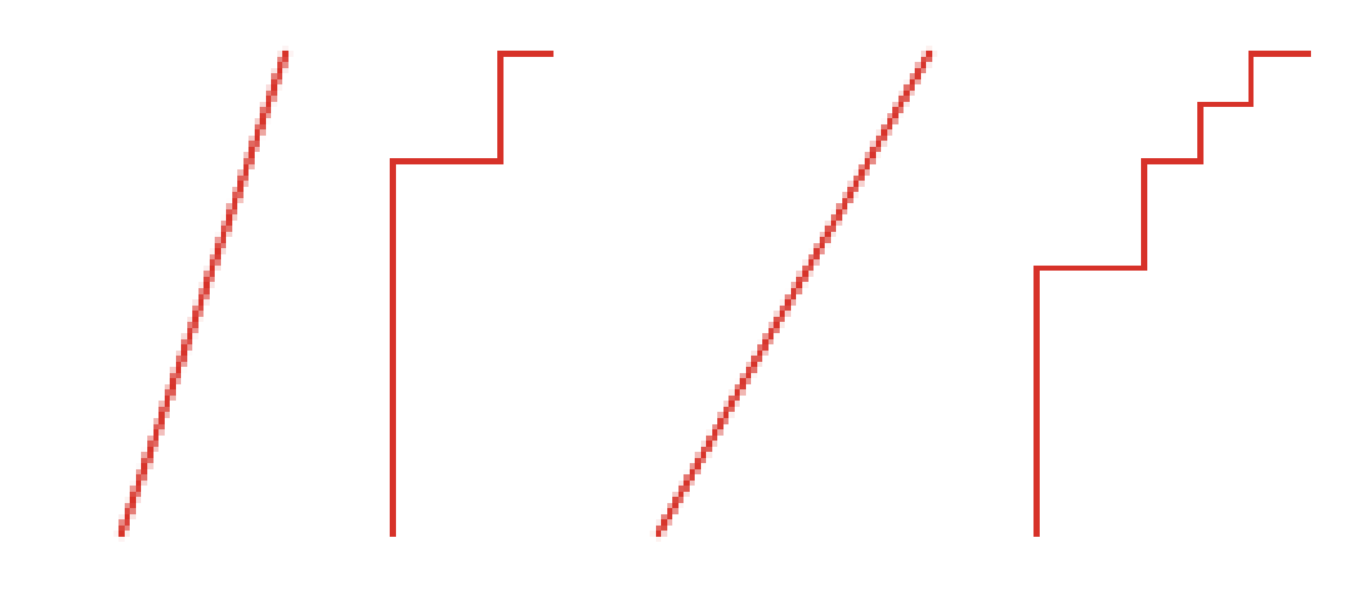
\includegraphics[width=\columnwidth]{assets/diagonal_path.png} 
    \caption{Two pairs of straightened (left) and not straightened-paths (right)}
    \label{fig:straightened_path}
\end{figure}

\begin{figure}[H]
    \centering
    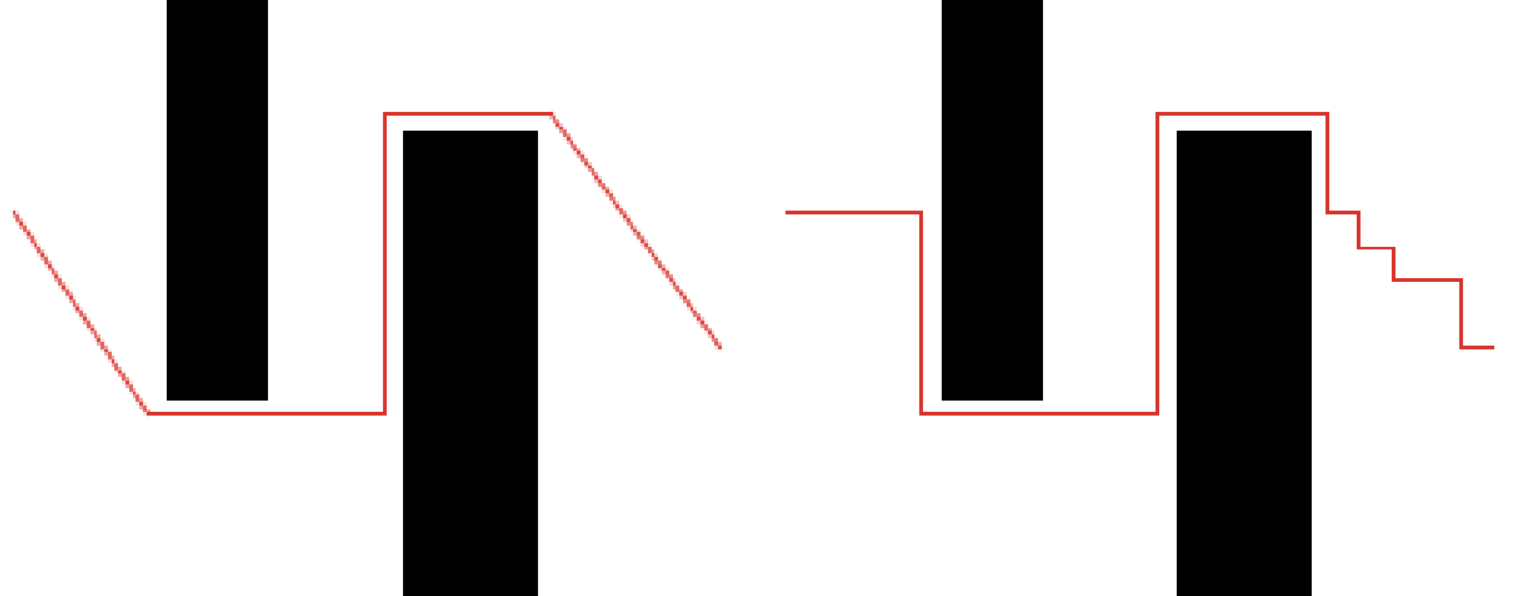
\includegraphics[width=\columnwidth]{assets/obstacle_path.png}
    \caption{A straightened (left) and not straightened path (right) around obstacles}
    \label{fig:straightened_path_around_obstacle}
\end{figure}

As you can see, in \autoref{fig:straightened_path_around_obstacle}, the straightened path is not optimal. It is impossible to know a priori if a path will be optimized or not. One could theorize an approach that leverages the one used above to improve it further. At the time, the only solution we envisioned would be to brute force the set of all straightenings one could do by straightening in a different order than that shown in \autoref{alg:straigthen-path-algorithm}. Alternatively, a completely different method of path-finding that eliminates the need for straightening could have been developed. In \textit{A*}, instead of adjacency being only the four patches with which an edge is shared, it could be every patch that forms a straight path from the given patch. This approach was ultimately not adopted out of fear of being too computationally heavy to calculate the neighbors. \\

For the straightening step, the function \textit{Is-Straight} is used. It is paramount, for it is what determines if a certain path (or sub-path) is straight. It takes into account the size of the passenger. The algorithm's intuition is that the passengers' path (and its volume) is approximated by a rectangle (in whatever orientation) and intersected with any possible obstacles that the passenger would collide with. Implementation-wise, the start and end of the path are checked for collisions independently. The rectangle intersection is, in turn, done by \textit{stepping} from the start to the end. The size of the step is linked to the precision of this approach: a bigger step means a smaller precision. In each step, a set of points is verified for possible collisions.\\

\begin{figure}[H]
    \centering
    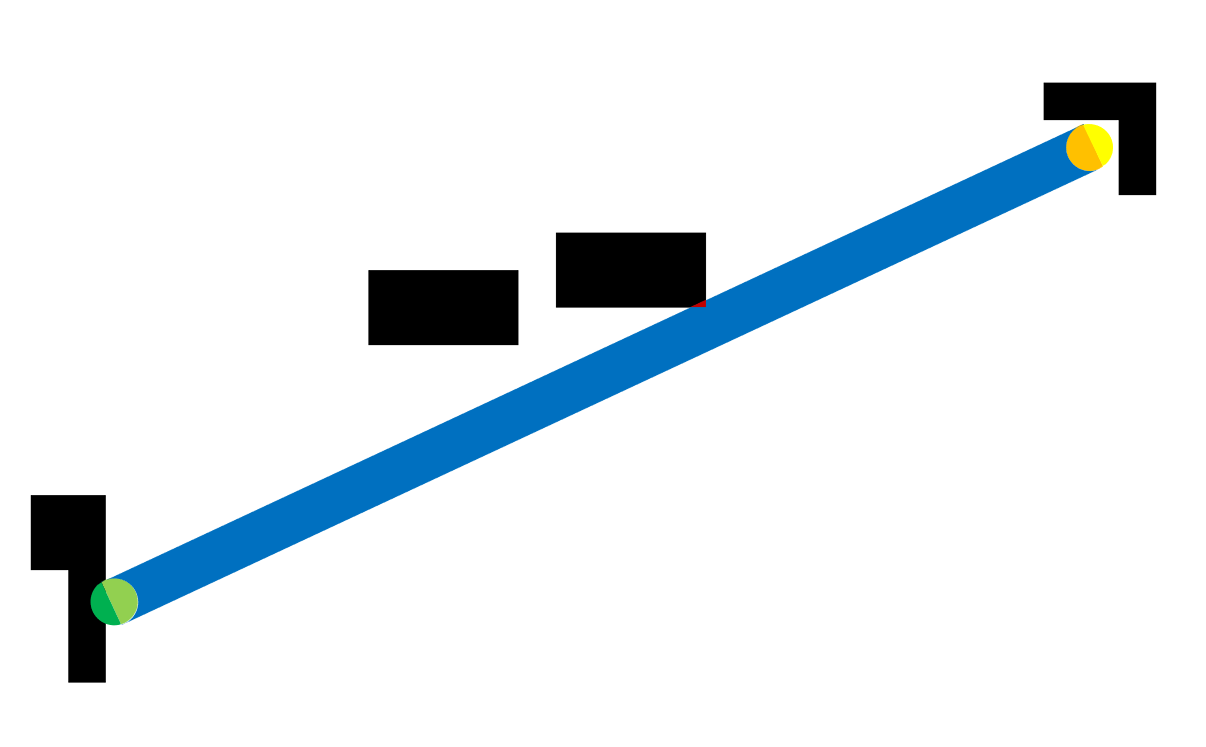
\includegraphics[width=\columnwidth]{assets/is-straight.png}
    \caption{Illustration of Is-Straight algorithm. Obstacles (black), passenger at start (green/light green circle), passenger at end (yellow/orange circle), passenger's path (blue rectangle), representation of collision (red), overlap of start and end with passenger's path (lime and orange semicircle, respectively)}
    \label{fig:is_straight}
\end{figure}

\begin{figure}[H]
    \centering
    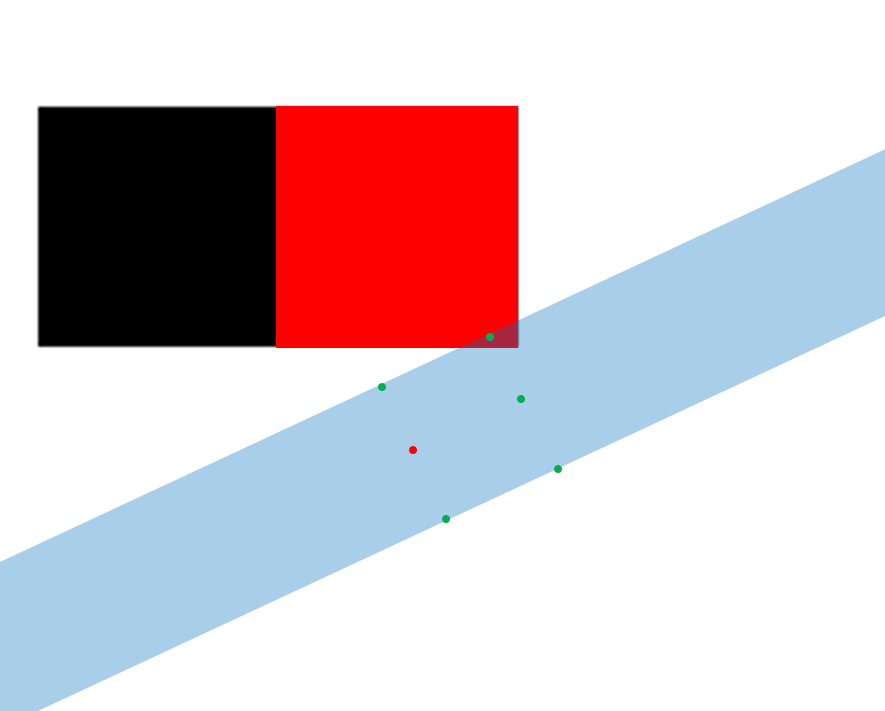
\includegraphics[width=\columnwidth]{assets/is-straight-step.png}
    \caption{Illustration of a step of Is-Straight algorithm. Obstacle (black), passenger's path (light blue), passenger's center in i-th step (red circle), passenger's collision verification points in i-th step (green circles), path with collision (red square)}
    \label{fig:is_straight_step}
\end{figure}

In \autoref{fig:is_straight}, a representation of the algorithm can be seen. The intersection of the passenger at the end of the path with an obstacle would mean the path is not straight. If that were not the case, the path's intersection with an obstacle would also yield the same result. This is achieved as is seen in \autoref{fig:is_straight_step}. Since one of the collision-verified points lies within the obstacle (a straightforward operation in NetLogo), there is indeed a collision. Note that, with a different step, there is a chance the collision is not detected.

\subsection {Passengers' path-finding}

To improve the scalability of a run by allowing a great number of passengers, passengers' path-finding leverages the preexisting static path-finding.  \\
Given the fact that a passenger most often wants to transition between platforms, it would be impossible for a naive path-finding algorithm in a 2d environment to work, given there are no patches that are neighbors with other floors and different platforms are physically separated from each other. To use said approach, interpreting the portals as patches that neighbor other floors would allow for the path-finding to proceed. However, the heuristic functions for \textit{A*} would have to take floors into account, making it not as trivial, and path-finding in the new floor would increase the size of the path-finding. The solution adopted is to separate the path-finding on a platform and between platforms. To find the shortest path that traverses multiple platforms, we first calculate the remaining platform paths and use that to find the path between the platforms.\\

The remaining platform paths consist of, for each passenger, path-finding from the passenger's source to the portals in the source's platform and from the passenger's destination to the portals in the destination's platform. To do this, instead of rerunning the path-finding algorithm described in \autoref{sec:methods_materials_static_pathfinding}, which would be time-consuming for a large number of passengers, we are going to reuse the already found paths and try to adapt them to the position of the passenger. \\

In the case of the path between the source and one of the portals, we consider the path already found between the centroid of the point of interest the source belongs to (remember, a source is a cell of a point of interest and not its centroid) and the portal. This path is an ordered list of positions. From the first to the second position, there is a straight path; the second position is where a "bend" is located, followed by another straight segment to the third position. We assume that the distance from the cell to the centroid of the point of interest is not significant and, therefore, said bend would still apply would we rerun the path-finding algorithm. Therefore, we attempt to fit the already-found path to the new cell. To do this, we verify if the path from the source to the second position is a straight path, using the \textit{Is-Straight} described in \autoref{sec:methods_materials_static_pathfinding}. If so, then the new path has been found. If not, then we choose the next point in the segment from the second position to the centroid of the point of interest until a path from the source to the chosen point is straight. Analogously for the destination. \\

\begin{figure}
    \centering
    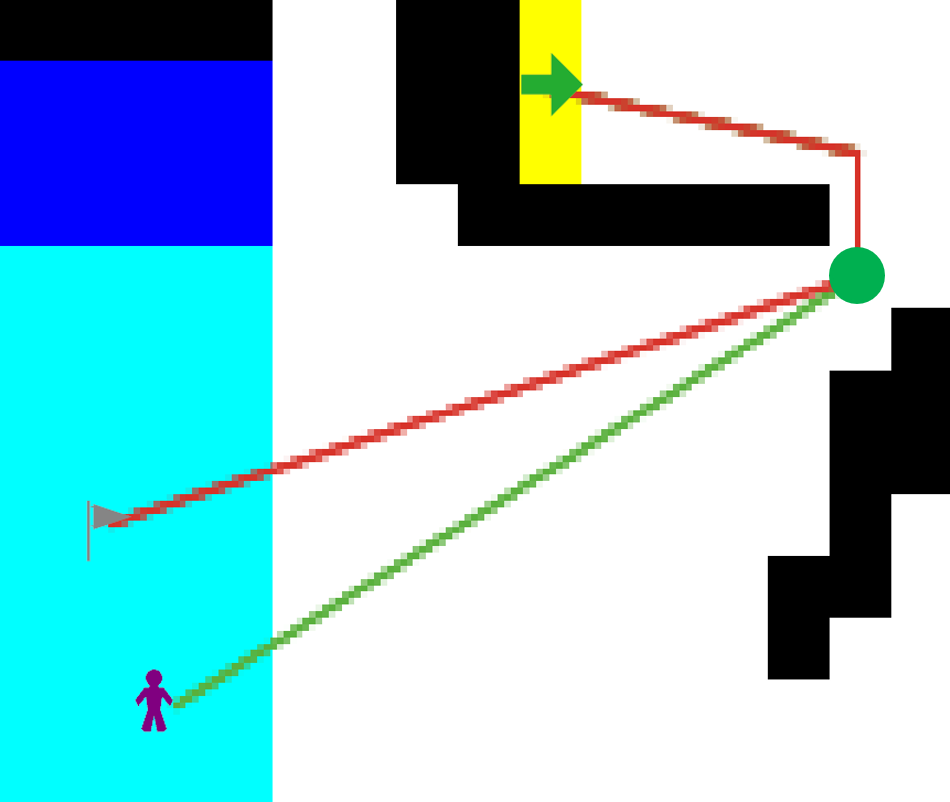
\includegraphics[width=\columnwidth]{assets/merge_path_straight.png}
    \caption{Merging paths. The pre-calculated path (red line), new segment that is merged (green line), second point (green circle), point of interest centroid (gray flag), and passenger (purple person)}
    \label{fig:merge_path_straight}
\end{figure}

\begin{figure}
    \centering
    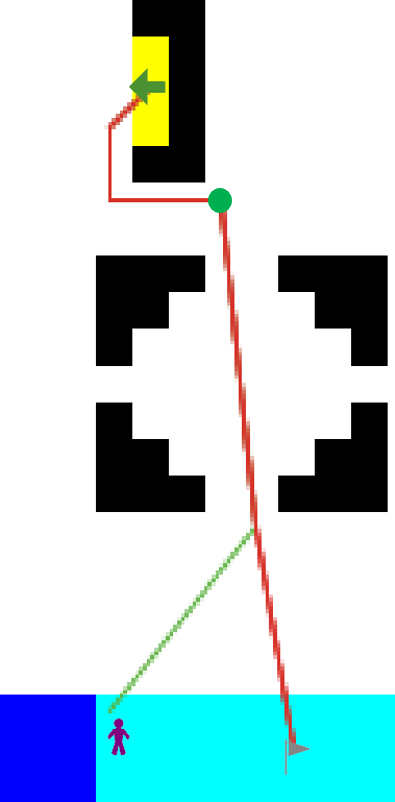
\includegraphics[width=\columnwidth]{assets/merge_path_not_straight.png}
    \caption{Merging paths. The pre-calculated path (red line), new segment that is merged (green line), second point (green circle), point of interest centroid (gray flag), and passenger (purple person)}
    \label{fig:merge_path_not_straight}
\end{figure}
In \autoref{fig:merge_path_straight} and \autoref{fig:merge_path_not_straight}, two examples of this path merging can be seen. In \autoref{fig:merge_path_not_straight}, as there wasn't a straight path from the source to the second point, the merge segment had to be calculated and doesn't connect straight to the second point.

For pathfinding between platforms, we use \textit{Dijkstra's} pathfinding algorithm, not on the environment's grid, but on a graph with certain entities as nodes. Those entities will be the source and destination cells for the passenger and every portal in the whole environment. Below there is a figure illustrating the final graph

\begin{figure}
    \centering
    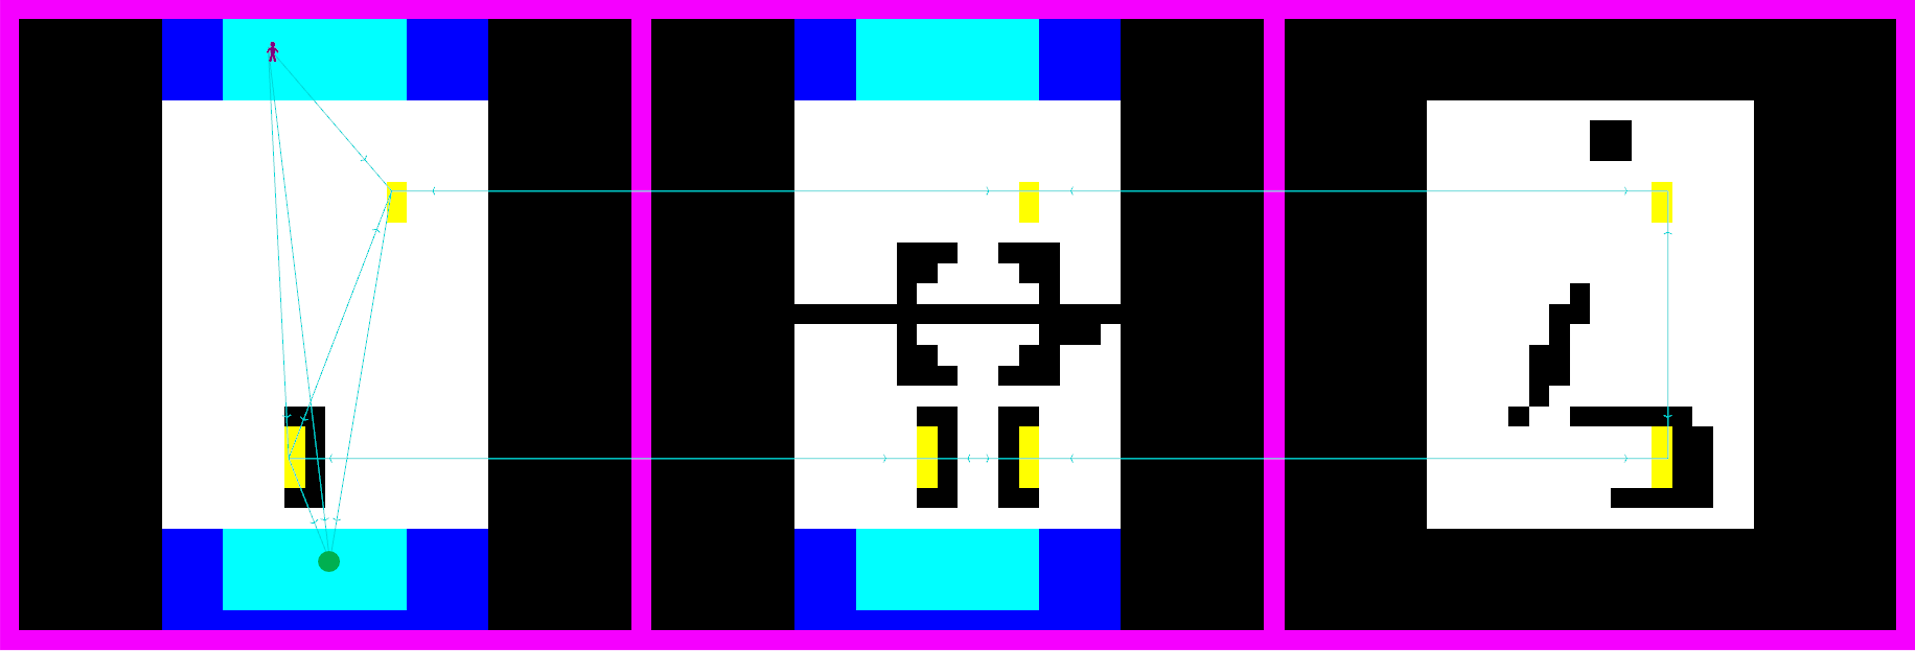
\includegraphics[width=\columnwidth]{assets/meta_pathfinding.png}
    \caption{Graph for path-finding between platforms. Edges of graph (Light blue lines) The portals, specifically stairs (yellow rectangles), passenger (purple person), and destination cell (green circle)}
    \label{fig:meta_pathfinding}
\end{figure}


\subsection {Collisions}

The collision between the passengers is done to minimize the superposition of passengers. It uses the Lennard-Jones potential described by the equation 
$$
V_{LJ}(r)=4\epsilon\left[\left(\frac{\sigma}{r}\right)^{12}-\left(\frac{\sigma}{r}\right)^6\right]
$$


\section{Results \& discussion}\label{sec:results_discussion}

To test the devised simulation, we ran a series of simulations in Trindade, a major station in Porto's metro system (Portugal). \autoref{fig:trindade} \\

\begin{figure}
    \centering
    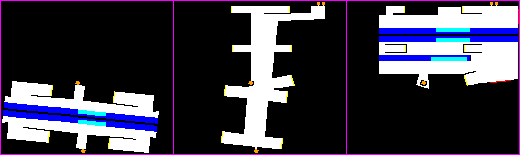
\includegraphics[width=\linewidth]{assets/trindade.png}
    \caption{Map for Trindade's station in NetLogo}
    \label{fig:trindade}
\end{figure}

We ran the following scenarios:

\begin{itemize}
    \item Normal
    \item No elevators
    \item Only one set of stairs per train
    \item Longer trains
    \item With escalators
\end{itemize}

For each scenario, we ran with a passenger load of 150 and 300. The metrics collected are listed below. In \autoref{sec:annexes} all of the tables with the metrics by experiment are listed. For each metric, a simple statistical analysis was performed.
\begin{itemize}
    \item Number of ticks: The number of ticks that it takes to run the experiment and for every passenger to reach their destination \ref{annex:tick}
    \item Distance per tick: The distance a passenger travels in a tick. By definition should be 0.3 units \ref{annex:tick_distance}
    \item Total distance: The total distance traveled by a passenger to reach their destination.  \ref{annex:distance}
    \item Crowdedness: The number of other passengers inside the given radius. \ref{annex:crowdedness_0.8}, \ref{annex:crowdedness_1}, \ref{annex:crowdedness_1.2}, \ref{annex:crowdedness_1.4}
\end{itemize}

When analysing the number of ticks of each experiment, we can see that not always does the experiment of 300 passengers take more steps to run. Additionally, the scenarios with no elevators or a single set of stairs do increase the number of ticks, as expected, since passengers will not always be able to take what would otherwise be the shortest path. There doesn't seem to be a great difference between the base scenario and the scenario with escalators, which leads us to conclude that maybe the shortest path does not include the escalators. (or if it does, there is no significant benefit). One thing to notice is that there seems to have been some abnormal behavior in experiments \textit{trindade-300} and \textit{trindade-single-stairs} as is seen by the \textit{max} column, which presents a much higher value. The percentiles are still within reason so we can interpret those values as outliers.

When it comes to the tick distance, the \textit{max} column is where we should focus on. A tick distance higher than 0.3 happens when the collision mechanisms push a passenger out of the way. A 75th percentile of 0.3 is therefore expected as collisions are not that frequent. The higher number of passengers and scenarios with less pathing alternatives leading to an, even if slight, increase in the maximum amount is expected but inconclusive. To be certain, we'd need to have higher percentiles of the data to see if this relation holds not only for the tick with the maximum distance, but for the ticks that employ some collision mechanism.

When it comes to totally distance travelled, mean values for each scenario are according to the hypothesis that less available pathing alternatives lead to worse outcomes. The scenarios \textit{trindade}, \textit{trindade-long-trains}, and \textit{trindade-escalators} having the same paths available have a similar mean distance traveled, where as \textit{trindade-no-elevators} has a higher distance traveled, and \textit{trindade-single-stairs} higher even. Looking in particular at the scenario with single stairs, there is a 100 units difference between the experiment with 150 and 300 passengers. This distance could be explained by a worse starting position for a passenger. One thing to notice is that there is an almost perfect correlation between total distance and number of ticks. As such, referring back to the maximum value for the number of ticks in the \textit{trindade-300} experiment which isn't reflected in the maximum distance traveled, we could hypothesize that that passenger might have become stuck, maybe as a malfunctioning of the simulation.

When it comes to crowdedness metrics, we can see that the numbers for the experiments with double the number of passengers are more or less double that of the normal amount. This is to be expected. The metrics for the scenario with the long trains is significantly lower, which makes sense considering the starting positions of the passengers will be more spaced out. There appears to be little correlation between the other scenarios and the crowdedness otherwise, which could indicate that the starting position of the passengers is the critical criteria for the crowdedness of the experiment. The results for a crowdedness of 0.6 are mostly 0, meaning the radius is too low to obtain any relevant information.

We can see how the differences in the scenarios did not always reflect in the data as would be expected from intuition. This could mean that the simulation is not a truthful interpretation of the real world or that the scenarios presented present insights into the dynamics of people in a transit station.





% \begin{table*}
% \begin{tabular}{|c|c|c|c|cccc|}
% \hline
% \multirow{2}{*}{\textbf{Metric}} & \multirow{2}{*}{\textbf{Ticks}} & \multirow{2}{*}{\textbf{Tick Distance}} & \multirow{2}{*}{\textbf{Total Distance}} & \multicolumn{4}{c|}{\textbf{Crowdedness}}                                                                                \\ \cline{5-8} 
%                                  &                                 &                                         &                                          & \multicolumn{1}{c|}{\textbf{0.8}} & \multicolumn{1}{c|}{\textbf{1.0}} & \multicolumn{1}{c|}{\textbf{1.2}} & \textbf{1.4} \\ \hline
% mean                             & 464.710000                      & 0.297951                                & 138.460790                               & \multicolumn{1}{c|}{0.001160}     & \multicolumn{1}{c|}{0.203689}     & \multicolumn{1}{c|}{0.397329}     & 0.457151     \\ \hline
% std                              & 204.348647                      & 0.024352                                & 61.119533                                & \multicolumn{1}{c|}{0.039845}     & \multicolumn{1}{c|}{0.541747}     & \multicolumn{1}{c|}{0.739537}     & 0.799496     \\ \hline
% min                              & 127.000000                      & 0.000000                                & 38.504057                                & \multicolumn{1}{c|}{0.000000}     & \multicolumn{1}{c|}{0.000000}     & \multicolumn{1}{c|}{0.000000}     & 0.000000     \\ \hline
% 25\%                             & 256.750000                      & 0.300000                                & 76.022187                                & \multicolumn{1}{c|}{0.000000}     & \multicolumn{1}{c|}{0.000000}     & \multicolumn{1}{c|}{0.000000}     & 0.000000     \\ \hline
% 50\%                             & 479.000000                      & 0.300000                                & 141.865455                               & \multicolumn{1}{c|}{0.000000}     & \multicolumn{1}{c|}{0.000000}     & \multicolumn{1}{c|}{0.000000}     & 0.000000     \\ \hline
% 75\%                             & 608.750000                      & 0.300000                                & 182.623531                               & \multicolumn{1}{c|}{0.000000}     & \multicolumn{1}{c|}{0.000000}     & \multicolumn{1}{c|}{1.000000}     & 1.000000     \\ \hline
% Max                              & 898.000000                      & 0.564923                                & 268.083006                               & \multicolumn{1}{c|}{3.000000}     & \multicolumn{1}{c|}{5.000000}     & \multicolumn{1}{c|}{6.000000}     & 6.000000     \\ \hline
% \end{tabular}
% \caption{Obtained results}
% \label{table:results}
% \end{table*}
\section{Conclusion} \label{sec:conclusion}
In this work, we used NetLogo to develop a simple pedestrian simulation of a transit station, with nothing more than an image as a guide for the modeling of said station. The implemented features would allow for the testing of most transit stations, given that common infrastructure was considered.
The results provided some promising results but were not sufficient to validate the model. Repetition of the experiments, a deeper analysis of the data, and other metrics could be employed to increase the value of the simulation.
In future work, passenger spawning could take a more realistic approach instead of passengers being all initialized at the start of the simulation. Additionally, path-finding algorithms that tackle the problems seen in \autoref{fig:straightened_path_around_obstacle} could be fruitful. Different types of agents, for example, agents with incomplete knowledge or different path preferences, were disregarded in this work. Studying other stations and how they compare in terms of metrics could provide insights into their relative performance. Despite some of the advantages of how \textit{turtles} and \textit{patches} are handled, NetLogo may not be the most suited tool for more extensive work in this area. Nonetheless, the methodology and algorithms developed may still provide guidance on how to implement a different system from scratch.

\printbibliography 
\section{Annexes}\label{sec:annexes}


\begin{table*}
% \makebox[\textwidth]{%
    \begin{tabular}{|c|cccccccc|}
      & mean & std & min & 25\% & 50\% & 75\% & max \\
    trindade  & 506.55 & 184.89 & 133.00 & 430.75 & 537.00 & 626.00 & 873.00 \\
    trindade-300  & 515.65 & 190.14 & 141.00 & 415.50 & 556.00 & 617.00 & 1352.00 \\
    trindade-long-trains  & 492.73 & 199.75 & 144.00 & 299.25 & 533.00 & 622.50 & 902.00 \\
    trindade-long-trains-300  & 504.73 & 174.67 & 131.00 & 370.25 & 556.50 & 617.00 & 896.00 \\
    trindade-no-elevators  & 596.83 & 229.77 & 120.00 & 528.00 & 625.00 & 751.25 & 1040.00 \\
    trindade-no-elevators-300  & 626.60 & 225.73 & 126.00 & 531.00 & 645.50 & 763.25 & 1070.00 \\
    trindade-single-stairs  & 722.95 & 305.63 & 157.00 & 619.25 & 777.00 & 927.00 & 1393.00 \\
    trindade-single-stairs-300  & 604.53 & 228.16 & 137.00 & 521.00 & 631.00 & 750.25 & 1053.00 \\
    trindade-escalators  & 511.70 & 192.74 & 145.00 & 438.00 & 537.00 & 625.75 & 886.00 \\
    trindade-escalators-300  & 496.96 & 180.59 & 138.00 & 425.00 & 536.00 & 597.50 & 914.00 \\
    \end{tabular}

% }
\caption{Statistics on the number of ticks for each of the experiments}
\label{annex:tick}  
\end{table*}

\begin{table*}

% \makebox[\textwidth]{%
    \begin{tabular}{|c|cccccccc|}
     & count & mean & std & min & 25\% & 50\% & 75\% & max \\
    trindade & 75983.00 & 0.30 & 0.02 & 0.00 & 0.30 & 0.30 & 0.30 & 0.55 \\
    trindade-300 & 154696.00 & 0.30 & 0.03 & 0.00 & 0.30 & 0.30 & 0.30 & 0.60 \\
    trindade-long-trains & 73910.00 & 0.30 & 0.02 & 0.00 & 0.30 & 0.30 & 0.30 & 0.55 \\
    trindade-long-trains-300 & 151418.00 & 0.30 & 0.02 & 0.00 & 0.30 & 0.30 & 0.30 & 0.72 \\
    trindade-no-elevators & 89524.00 & 0.30 & 0.01 & 0.04 & 0.30 & 0.30 & 0.30 & 0.58 \\
    trindade-no-elevators-300 & 187979.00 & 0.30 & 0.01 & 0.04 & 0.30 & 0.30 & 0.30 & 0.60 \\
    trindade-single-stairs & 108443.00 & 0.30 & 0.01 & 0.00 & 0.30 & 0.30 & 0.30 & 0.56 \\
    trindade-single-stairs-300 & 181358.00 & 0.30 & 0.01 & 0.02 & 0.30 & 0.30 & 0.30 & 0.58 \\
    trindade-escalators & 76755.00 & 0.31 & 0.09 & 0.00 & 0.30 & 0.30 & 0.30 & 0.90 \\
    trindade-escalators-300 & 149088.00 & 0.31 & 0.09 & 0.00 & 0.30 & 0.30 & 0.30 & 1.01 \\
    \end{tabular}
% }
\caption{Statistics on the distance traveled in each tick for each of the experiments}
\label{annex:tick_distance}

\end{table*}

\begin{table*}
% \makebox[\textwidth]{%
    \begin{tabular}{|c|cccccccc|}
      & mean & std & min & 25\% & 50\% & 75\% & max \\
    trindade  & 150.91 & 55.35 & 39.45 & 126.78 & 160.35 & 186.80 & 260.37 \\
    trindade-300  & 152.61 & 54.36 & 42.14 & 122.74 & 164.21 & 184.42 & 261.64 \\
    trindade-long-trains  & 146.91 & 59.63 & 43.02 & 89.77 & 158.80 & 185.58 & 269.82 \\
    trindade-long-trains-300  & 150.30 & 52.24 & 39.11 & 109.93 & 166.42 & 183.99 & 267.25 \\
    trindade-no-elevators  & 179.03 & 68.91 & 36.18 & 158.66 & 187.01 & 225.32 & 311.86 \\
    trindade-no-elevators-300  & 187.86 & 67.68 & 37.40 & 159.77 & 193.72 & 228.52 & 320.38 \\
    trindade-single-stairs  & 216.79 & 91.81 & 47.02 & 185.98 & 232.98 & 278.26 & 418.16 \\
    trindade-single-stairs-300  & 181.24 & 68.40 & 40.84 & 156.70 & 189.19 & 224.80 & 316.42 \\
    trindade-escalators  & 158.36 & 60.68 & 43.15 & 129.36 & 173.33 & 193.04 & 264.95 \\
    trindade-escalators-300  & 154.30 & 57.44 & 41.47 & 126.23 & 170.84 & 190.38 & 273.52 \\
    \end{tabular}
% }
\caption{Statistics on the total distance traveled for each of the experiments}
\label{annex:distance}

\end{table*}


\begin{table*}
% \makebox[\textwidth]{%
    \begin{tabular}{|c|cccccccc|}
      & mean & std & min & 25\% & 50\% & 75\% & max \\
    trindade  & 0.00 & 0.07 & 0.00 & 0.00 & 0.00 & 0.00 & 4.00 \\
    trindade-300  & 0.02 & 0.21 & 0.00 & 0.00 & 0.00 & 0.00 & 6.00 \\
    trindade-long-trains  & 0.00 & 0.04 & 0.00 & 0.00 & 0.00 & 0.00 & 3.00 \\
    trindade-long-trains-300  & 0.01 & 0.20 & 0.00 & 0.00 & 0.00 & 0.00 & 6.00 \\
    trindade-no-elevators  & 0.00 & 0.02 & 0.00 & 0.00 & 0.00 & 0.00 & 1.00 \\
    trindade-no-elevators-300  & 0.01 & 0.10 & 0.00 & 0.00 & 0.00 & 0.00 & 3.00 \\
    trindade-single-stairs  & 0.00 & 0.05 & 0.00 & 0.00 & 0.00 & 0.00 & 3.00 \\
    trindade-single-stairs-300  & 0.01 & 0.09 & 0.00 & 0.00 & 0.00 & 0.00 & 4.00 \\
    trindade-escalators  & 0.00 & 0.08 & 0.00 & 0.00 & 0.00 & 0.00 & 4.00 \\
    trindade-escalators-300  & 0.02 & 0.20 & 0.00 & 0.00 & 0.00 & 0.00 & 7.00 \\
    \end{tabular}
% }
\caption{Statistics on crowdedness at a radius of 0.8 for each of the experiments}
\label{annex:crowdedness_0.8}

\end{table*}


\begin{table*}
% \makebox[\textwidth]{%
    \begin{tabular}{|c|cccccccc|}
      & mean & std & min & 25\% & 50\% & 75\% & max \\
    trindade  & 0.28 & 0.63 & 0.00 & 0.00 & 0.00 & 0.00 & 5.00 \\
    trindade-300  & 0.66 & 1.01 & 0.00 & 0.00 & 0.00 & 1.00 & 8.00 \\
    trindade-long-trains  & 0.13 & 0.39 & 0.00 & 0.00 & 0.00 & 0.00 & 4.00 \\
    trindade-long-trains-300  & 0.40 & 0.78 & 0.00 & 0.00 & 0.00 & 1.00 & 9.00 \\
    trindade-no-elevators  & 0.22 & 0.53 & 0.00 & 0.00 & 0.00 & 0.00 & 4.00 \\
    trindade-no-elevators-300  & 0.67 & 0.96 & 0.00 & 0.00 & 0.00 & 1.00 & 5.00 \\
    trindade-single-stairs  & 0.26 & 0.59 & 0.00 & 0.00 & 0.00 & 0.00 & 5.00 \\
    trindade-single-stairs-300  & 0.68 & 0.93 & 0.00 & 0.00 & 0.00 & 1.00 & 6.00 \\
    trindade-escalators  & 0.30 & 0.67 & 0.00 & 0.00 & 0.00 & 0.00 & 6.00 \\
    trindade-escalators-300  & 0.57 & 0.98 & 0.00 & 0.00 & 0.00 & 1.00 & 9.00 \\
    \end{tabular}
% }
\caption{Statistics on crowdedness at a radius of 1 for each of the experiments}
\label{annex:crowdedness_1}

\end{table*}

\begin{table*}
% \makebox[\textwidth]{%
    \begin{tabular}{|c|cccccccc|}
      & mean & std & min & 25\% & 50\% & 75\% & max \\
    trindade  & 0.51 & 0.80 & 0.00 & 0.00 & 0.00 & 1.00 & 7.00 \\
    trindade-300  & 1.02 & 1.20 & 0.00 & 0.00 & 1.00 & 2.00 & 10.00 \\
    trindade-long-trains  & 0.27 & 0.55 & 0.00 & 0.00 & 0.00 & 0.00 & 5.00 \\
    trindade-long-trains-300  & 0.66 & 0.98 & 0.00 & 0.00 & 0.00 & 1.00 & 12.00 \\
    trindade-no-elevators  & 0.57 & 0.77 & 0.00 & 0.00 & 0.00 & 1.00 & 4.00 \\
    trindade-no-elevators-300  & 1.07 & 1.12 & 0.00 & 0.00 & 1.00 & 2.00 & 6.00 \\
    trindade-single-stairs  & 0.51 & 0.75 & 0.00 & 0.00 & 0.00 & 1.00 & 6.00 \\
    trindade-single-stairs-300  & 1.03 & 1.09 & 0.00 & 0.00 & 1.00 & 2.00 & 6.00 \\
    trindade-escalators  & 0.55 & 0.88 & 0.00 & 0.00 & 0.00 & 1.00 & 7.00 \\
    trindade-escalators-300  & 0.91 & 1.21 & 0.00 & 0.00 & 0.00 & 1.00 & 10.00 \\
    \end{tabular}
% }
\caption{Statistics on crowdedness at a radius of 1.2 for each of the experiments}
\label{annex:crowdedness_1.2}

\end{table*}

\begin{table*}
% \makebox[\textwidth]{%
    \begin{tabular}{|c|cccccccc|}
      & mean & std & min & 25\% & 50\% & 75\% & max \\
    trindade  & 0.59 & 0.90 & 0.00 & 0.00 & 0.00 & 1.00 & 8.00 \\
    trindade-300  & 1.21 & 1.36 & 0.00 & 0.00 & 1.00 & 2.00 & 14.00 \\
    trindade-long-trains  & 0.34 & 0.63 & 0.00 & 0.00 & 0.00 & 1.00 & 6.00 \\
    trindade-long-trains-300  & 0.80 & 1.13 & 0.00 & 0.00 & 0.00 & 1.00 & 15.00 \\
    trindade-no-elevators  & 0.64 & 0.82 & 0.00 & 0.00 & 0.00 & 1.00 & 5.00 \\
    trindade-no-elevators-300  & 1.24 & 1.24 & 0.00 & 0.00 & 1.00 & 2.00 & 7.00 \\
    trindade-single-stairs  & 0.58 & 0.82 & 0.00 & 0.00 & 0.00 & 1.00 & 7.00 \\
    trindade-single-stairs-300  & 1.21 & 1.20 & 0.00 & 0.00 & 1.00 & 2.00 & 7.00 \\
    trindade-escalators  & 0.66 & 1.00 & 0.00 & 0.00 & 0.00 & 1.00 & 8.00 \\
    trindade-escalators-300  & 1.08 & 1.41 & 0.00 & 0.00 & 1.00 & 2.00 & 12.00 \\
    \end{tabular}
% }
\caption{Statistics on crowdedness at a radius of 1.4 for each of the experiments}
\label{annex:crowdedness_1.4}

\end{table*} 

\end{document}
